\documentclass[11pt, a4paper, oneside]{article}

\usepackage{indentfirst}

% hifenização e outras especificações para português
\usepackage[portuguese]{babel}

% hiperligações
\usepackage{hyperref}
\hypersetup{colorlinks=true, urlcolor=blue, linkcolor=black}

% escrever acentos e coisas do género sem que o latex se desoriente
\usepackage[utf8]{inputenc}

% para ter imagens, depois define a directoria de imagens
\usepackage{graphicx}
\graphicspath{{./imagens/}}

\usepackage[labelformat=simple]{caption}
\usepackage[labelformat=empty]{subcaption}

% para ter a informação de quantas páginas tem o documento
\usepackage{lastpage}

% definir o cabeçalho e rodapé
\usepackage{fancyhdr}
\pagestyle{fancy}
\fancyhead[L]{\small{Not Another Wikipedia Parser}}
\fancyhead[R]{\small{Processamento de Linguagens}}

% ter enumerações alinhadas
\usepackage{enumitem}

% escrever algoritmos
\usepackage[algoruled]{algorithm2e}

% mais cores predefinidas
\usepackage[usenames,dvipsnames]{color}

% definir comandos especiais
\newcommand\doubleplus{+\kern-1.3ex+\kern0.8ex} %

\newcommand{\todo}[1] {\textcolor{BrickRed}{\begin{quote}#1\end{quote}}}

%\usepackage{listings}


%%%%%%%%%%%%%%%%%%%%%%%%%%%%%%%%%%%%%%%%%%%%%%
%% inicio do documento
\begin{document}
\title{Not Another Wikipedia Parser\\
\begin{normalsize}
Processamento da Wikipédia - Variante 1
\end{normalsize}}
\date{\today\\Universidade do Minho}
\author{
  Bruno Ferreira\\
  {\small A61055}\\
  \and
  Cláudia Oliveira\\
  {\small A60987}\\
  \and
  Vanessa Campos\\
  {\small A54801}\\
}

\maketitle

\begin{figure}[h]
\begin{center}

\includegraphics[width=0.4\linewidth]{logo}
\end{center}
\end{figure}


\begin{abstract}

  O presente trabalho foi desenvolvido no âmbito da Unidade Curricular de Processamento de Linguagens e tem como principal objetivo descrever o processo de desenvolvimento de um analisador léxico da \textit{Wikipédia}. Ao longo deste relatório iremos explicar as estruturas de dados que foram implementadas para o desenvolvimento deste trabalho, bem como todas as decisões que foram tomadas.

\end{abstract}
\newpage

\tableofcontents
\listoffigures 

\newpage
\section{Introdução}

Atualmente a \textit{Wikipédia} é a maior base de dados de conhecimento livre online e disponível em várias línguas. Neste contexto, pretende-se desenvolver um Processador de Texto, exportado da \textit{Wikipédia} e gerar a página html com os dados mais relevantes contidos nessa página, utilizando a ferramenta Flex. 
Neste trabalho foi necessário implementar Expressões Regulares de modo a retirar informação relevante. Para isto foi necessário encontrar padrões que nos ajudem a descobrir o tipo de informação que estamos à procura e que é útil no contexto deste caso de estudo.


\newpage
\section{Desenvolvimento}

\subsection{Contextualização do Problema}

Flex é uma ferramenta para gerar automaticamente analisadores léxicos, isto é, programas que reconhecem padrões léxicos num texto. O Flex é uma evolução da ferramenta Lex, mas com a caraterística de ser mais rápido que este (Fast Lex). Lex foi desenvolvido por M.E. Lesk e E. Shmidt (Bell Laboratories - ATT) enquanto que o Flex é um produto da Free Software Foundation, Inc. Ao contrário do programador que escreve manualmente um programa que realize a identificação de padrões numa entrada, o uso do Flex/Lex permite que sejam apenas especificados os padrões desejados e as ações necessárias para processá-los. Para que Flex/Lex reconheçam padrões no texto, tais padrões devem ser descritos através de expressões regulares. A ferramenta Flex é ótima para a realização deste trabalho uma vez que nos permite analisar o conteúdo específico, através de expressões regulares de determinada informação de texto.

\subsection{Processamento da \textit{Wikipédia}}
Neste primeiro trabalho de Processamento de Linguagens foi-nos proposto escolher um de vários enunciados propostos. Após uma análise de cada um deles, o nosso grupo optou por escolher o tema de Processamento da \textit{Wikipédia}. O objetivo deste projeto é criar um programa utilizando a ferramenta Flex que analise o conteúdo de uma página XML da \textit{Wikipédia} e retire informações como:
\begin{itemize}
\item título;
\item autor;
\item data;
\item n.º de links internos;
\item n.º de links externos;
\item n.º de secções.
\end{itemize}
e criar uma página HTML com essas informações. Para isso é necessário exportar uma ou mais páginas usando o \textit{Special Export} disponível em \\\textbf{http://pt.wikipedia.org/wiki/Especial:Exportar} (ou \\\textbf{http://en.wikipedia.org/wiki/Special:Export} para a versão inglesa).

De momento, a nossa aplicação apenas interpreta corretamente páginas da Wikipédia em inglês.
\newpage

\subsection{Enunciado}

De uma maneira geral, para este trabalho pretende-se desenvolver os seguintes pontos:
\begin{itemize}
\item Especificar padrões de frases que se quer encontrar no texto fonte através de ERs.
\item Identificar as ações semânticas a realizar como reação ao reconhecimento de cada um desses padrões
\item Identificar estruturas de dados globais que possa eventualmente precisar para armazenar temporariamente a informação que se vai extraindo ou que se vai construindo à medida que o processamento avança.
\item Desenvolver um Processador de Texto para fazer reconhecimento dos padrões identificados e proceder à transformação pretendida, com recurso do Flex.
\end{itemize}

\subsection{Descrição do Problema}

Usando o \textbf{Especial Export} pretende-se exportar o conteúdo da \textit{Wikipédia} e com o recurso do Flex implementar um processador de texto que deverá produzir uma página \textbf{html} com as seguintes informações sobre as páginas especificadas no ficheiro XML:

\begin{itemize}
\item Título;
\item Autor da última revisão;
\item Data da última revisão;
\item Número de links internos, e explicitar quais;
\item Número de links externos, e explicitar quais;
\item Número de secções, e explicitar quais;
\item Opcional: raciocinar sobre como mostrar na página \textit{html} o conteúdo original do artigo.
\end{itemize}

\newpage

\subsection{Desenvolvimento do Programa}

\subsubsection{Estrutura de Dados}

Após termos analisado o ficheiro XML da \textit{Wikipédia} verificou-se que era necessário estruturar a informação encontrada nesses ficheiros. Essa informação é guardada em estruturas de dados que aqui vão ser expostas e explicadas. 

Decidimos que se ia guardar a informação sobre as páginas e no fim toda a informação ia ser escrita como output do programa. Concordámos que a forma mais simples de manter a informação sobre as páginas é uma lista ligada. Cada página tem informações como o título e o autor, e conjuntos de hiperligações internas, hiperligações externas e secções. Estes conjuntos são todos de fácil representação com listas ligadas, assim sendo criámos uma lista ligada genérica e usámos essa lista como estrutura de suporte a todos os conjuntos de informação.

O elemento da lista ligada genérica (do tipo Elemento) consiste apenas num apontador para os dados e num apontador para o próximo elemento da lista.
No que diz respeito às páginas, o tipo do apontador dados é \emph{Pagina}, como é possível ver na seguinte imagem.

\begin{figure}[h]
\begin{center}
\includegraphics[width=0.9\linewidth]{paginas}
\caption{Estrutura de Dados de Páginas}
\end{center}
\end{figure}

Para armazenar a informação dos componentes de cada página do XML, foi criado a seguinte estrutura de dados: \\
\begin{figure}[h]
\begin{center}
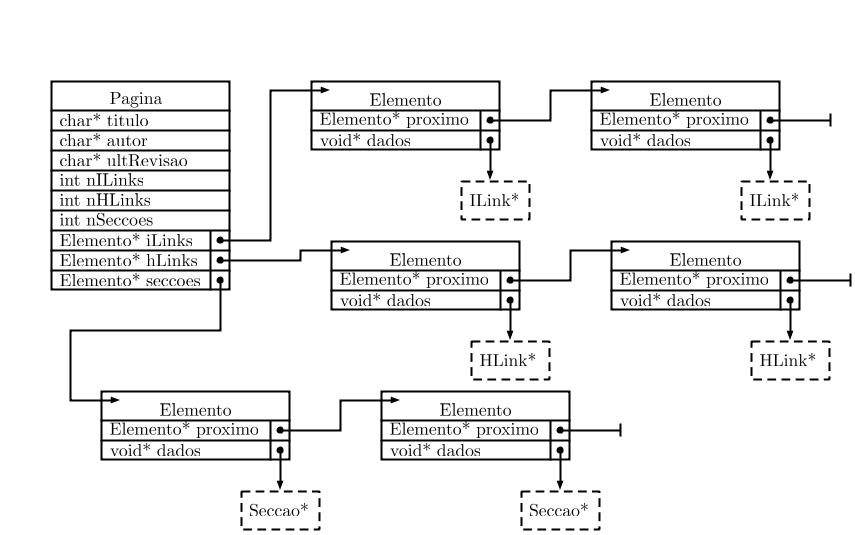
\includegraphics[width=0.9\linewidth]{pagina}
\caption{Estrutura de Dados de Página}
\end{center}
\end{figure}

Nos campos de estrutura da página armazena-se a seguinte informação:
\begin{itemize}

\item \textit{titulo} guarda o título da página da\textit{Wikipédia};
\item \textit{autor} guarda o autor da página;
\item \textit{ultRevisao} guarda a data da última revisão;
\item \textit{nILinks} guarda o número de links internos encontrados;
\item \textit{nHLinks} guarda o número de links externos encontrados;
\item \textit{nSeccões} guarda o número de secções encontradas;
\item \textit{iLikins} é o apontador para a lista ligada que guarda a informação dos links internos;
\item \textit{hLinks} é o apontador para a lista ligada que guarda a informação dos links externos;
\item \textit{seccoes} é apontador para a lista ligada que guarda a informação das secções da página.
\end{itemize}


\newpage
\subsubsection{Flex e Expressões Regulares}

Nesta secção iremos fazer uma abordagem as Expressões Regulares que foram desenvolvidas no contexto da resolução deste projeto. Utilizaram-se as seguintes condições de contexto:

\begin{verbatim}
%x page
%x title
%x revision
%x timestamp
%x contributor
%x username
%x text

%x ilink1
%x ilink2
%x ilink3
%x ilink4
%x hlink1
%x hlink2
%x head1
%x head2
%x head3
%x head4
%x head5
%x head6


\end{verbatim}


Na primeira fase do documento \emph{flex} importamos as funções dos vários módulos, bem como a definição de variáveis globais que servirão de "suporte" a cada uma das suas estruturas. A variável \texttt{paginas} é a lista ligada onde será guardada toda a informação recolhida. As variáveis \texttt{ilink}, \texttt{hlink} e \texttt{pag} contêm a página, o link interno ou o link externo que está a ser construído, respetivamente.

\begin{verbatim}
%{
#include "paginas.h"
#include "pagina.h"
#include "ilink.h"
#include "hlink.h"

ILink* ilink = NULL;
HLink* hlink = NULL;
Pagina* pag = NULL;
Elemento* paginas = NULL;

%}

\end{verbatim}
Será feita uma breve descrição das expressões regulares desenvolvidas neste projeto. As expressões podem não estar na mesma ordem que estão no ficheiro para que seja mais fácil a sua explicação.

Começando por explicar as primeiras expressões regulares que foram implementadas: 

\begin{verbatim}
"<page>"            {pag = pagina_create();
                     BEGIN page;
                    }
<page>"</page>"     {BEGIN 0;
                     paginas_add(paginas, pag);
                    }
\end{verbatim}

Quando se encontra a tag \texttt{<page>} inicia o estado page que dá início à interpretação dos dados da página. Por outro lado, quando encontra \texttt{</page>}, volta ao estado inicial e guarda a página na lista de páginas.

A função \texttt{pagina\_create()} permite inicializar a estrutura de dados que serve de suporte a uma página.

A função \texttt{paginas\_add} adiciona a página à lista ligada de páginas.

Note-se que no fim da recolha da informação sobre uma página, os conteúdos são guardados na lista ligada de páginas e, portanto, pode-se reutilizar a variável \texttt{pag} para guardar informações da página seguinte.

\begin{verbatim}
<page>"<title>"     BEGIN title;
<page>"<revision>"  BEGIN revision;
<title>"</title>"   BEGIN page;
<title>[^<]*        pagina_set_titulo(pag,yytext);
\end{verbatim}

Quando se está no estado page e é encontrada a tag \texttt{<title>}, inicia-se o estado título e é apanhado todo o texto até que seja encontrada a tag \texttt{</title>}. Após isto a informação é guarda no respetivo campo (neste caso campo título da estrutura página).

\begin{verbatim}
<page>"<revision>"         BEGIN revision;
<revision>"<timestamp>"    BEGIN timestamp;
<revision>"<contributor>"  BEGIN contributor;
\end{verbatim}

No caso de estarmos no estado page podemos encontrar a tag \texttt{revison}, que contém informações sobre a ultima revisão à página. Depois entrar no estado \texttt{revison} devem-se encontrar dois elementos XML: a \texttt{timestamp} e o \texttt{contributor}.

Primeiro encontrará a tag \texttt{timestamp}:

\begin{verbatim}
<timestamp>"</timestamp>"  BEGIN revision;
<timestamp>[^<]*           pagina_set_ultimaRevisao(pag, yytext);
\end{verbatim}

A tag \texttt{timestamp} dá informação relativa à data e hora da revisão.
Quando se encontra a tag de fecho da \texttt{timestamp} significa que todo o texto relativo à data e hora foi capturado e volta-se a estar dentro da tag \texttt{revision}.

A função \texttt{pagina\_set\_ultimaRevisao(Pagina* p, char* str)} preenche na estrutura da página o campo ultRevisao com a informação relativa da data e hora da revisão.


Segue-se a tag \texttt{contributor}:

\begin{verbatim}
<contributor>"<username>"      BEGIN username;
<contributor>"</contributor>"  BEGIN revision;

<username>"</username>"    BEGIN contributor;
<username>[^<]*            pagina_set_autor(pag, yytext);
\end{verbatim}

Dentro da tag \texttt{contributor} apenas nos interessa encontrar o nome do utilizador que fez a revisão. Portanto mudamos de estado, lemos o nome de utilizador de forma semelhante ao título (mas sabendo que o texto alvo está dentro da tag \texttt{username}) e usamos a função \texttt{pagina\_set\_autor(pag, yytext)} para guardar a informação recolhida. Depois temos regras para retroceder nos estados até estarmos novamente na tag \texttt{revision}.


Seguem-se agora expressões que permitem identificar conteúdos dentro do texto principal da página.

\begin{verbatim}
<revision>\<text.*?\>      BEGIN text;
<text>"</text>"            BEGIN revision;
<revision>"</revision>"    BEGIN page;
\end{verbatim}

Quando se está no estado revision, encontrando a tag \texttt{text} passamos ao estado que lhe corresponde e tem o mesmo nome. Esse estado termina quando se encontra a tag de término do elemento \texttt{text} do XML.

Depois de ler informações do elemento \texttt{text}, sabemos que não se segue mais informação relevante sobre a página e, portanto, resta-nos encontrar a tag de fim do elemento \texttt{revision} e passar ao estado \texttt{page} onde iremos depois encontrar a tag que marca o fim do elemento \texttt{page}.

Passamos agora a explicitar as expressões regulares que capturam informações sobre secções e hiperligações.


As seguintes expressões tratam de capturar informações sobre as secções da página:

\begin{verbatim}
<text>\n\=          BEGIN head1;
<text>\n\={2}       BEGIN head2;
<text>\n\={3}       BEGIN head3;
<text>\n\={4}       BEGIN head4;
<text>\n\={5}       BEGIN head5;
<text>\n\={6}       BEGIN head6;

<head1>[^\=]+  pagina_add_seccao(pag, seccao_create(yytext, 1));
<head2>[^\=]+  pagina_add_seccao(pag, seccao_create(yytext, 2));
<head3>[^\=]+  pagina_add_seccao(pag, seccao_create(yytext, 3));
<head4>[^\=]+  pagina_add_seccao(pag, seccao_create(yytext, 4));
<head5>[^\=]+  pagina_add_seccao(pag, seccao_create(yytext, 5));
<head6>[^\=]+  pagina_add_seccao(pag, seccao_create(yytext, 6));

<head1>\={1}                        BEGIN text;
<head2>\={2}                        BEGIN text;
<head3>\={3}                        BEGIN text;
<head4>\={4}                        BEGIN text;
<head5>\={5}                        BEGIN text;
<head6>\={4}                        BEGIN text;
\end{verbatim}

Podem ser apanhados 5 tipos de cabeçalhos, em que o 1 é o cabeçalho principal e a partir daqui os próximos são os sub cabeçalhos. A utilização do cabeçalho 1 é desaconselhada visto que é o formato utilizado para o título da página, mas incluí-mo-lo de qualquer forma.

A função \texttt{seccao\_create(char* str, int indentacao)} cria uma nova \texttt{Seccao} com o texto e tipo especificado e a função \texttt{pagina\_add\_seccao(Pagina* pagina, Seccao* seccao)} adiciona a secção à página.

O ultimo conjunto de regras faz com que se volte ao estado anterior (\texttt{texto}) depois de interpretar um cabeçalho de secção.



Relativamente às próximas regras, quando se encontra \texttt{[[} significa que temos um link interno que deve ser interpretado. Exceções a esta regra são links especiais começados por \texttt{[[File:} ou \texttt{[[Image:}, que não correspondem simplesmente a hiperligações, mas a conteúdos multimédia. Nos casos especiais pretende-se ignorar a tag de início do link para permitir a captura de links que estejam na descrição dos conteúdos multimédia.

A estrutura do link externo consiste apenas num conjunto de strings que permitem depois identificar as várias partes do link que foram capturadas. Esta estrutura pode ser consultada 

\begin{verbatim}
<text>"[[File:"     ;
<text>"[[Image:"    ;
<text>"[[":?        BEGIN ilink1;
\end{verbatim}

Ao ser encontrada uma hiperligação interna, o programa segue uma sequência de estados conforme identifica mais características do link.
\begin{verbatim}
<ilink1>[a-zA-Z]+:[^\]\(,\|]+  {ilink = ilink_create();
                                ilink_set_especial(ilink, yytext); 
                                BEGIN ilink2;}
\end{verbatim}

Quando é apanhada a expressão regular acima significa que foi apanhado um link que começa como, por exemplo, o link \texttt{[[Category:Salts]]}. Neste caso iria ser criado um novo link (com a função \texttt{ilink\_create()}) e a função \texttt{ilink\_set\_especial(ILink* ilink, char* str)} atribuiria a string \texttt{"Category"} ao campo \texttt{especial} e a string \texttt{"Salts"} ao campo \texttt{texto}.


\begin{verbatim}
<ilink1>[^\]\(,\|]+   {ilink = ilink_create();
                       ilink_set_texto(ilink, yytext);
                       BEGIN ilink2;}
\end{verbatim}

Quando é apanhada a expressão regular acima significa que foi apanhado um link que começa como, por exemplo, \texttt{[[Salts]]}. Neste caso iria ser criado um novo link (com a função \texttt{ilink\_create()}) e a função \texttt{ilink\_set\_texto(ILink* ilink, char* str)} atribuiria a string \texttt{"Salts"} ao campo \texttt{texto}.


\begin{verbatim}
<ilink2,ilink3>\]      {BEGIN ilink4;}
\end{verbatim}

Este caso existe porque em ambas as condições de contexto \texttt{ilink2} e \texttt{ilink3} é possível que o link termine. Qaundo isso acontece deve-se seguir para a condição de contexto \texttt{ilink4}.

\begin{verbatim}
<ilink2>\|               {BEGIN ilink3;}
\end{verbatim}

Ao estar na condição de contexto \texttt{ilink2} e encontrar o carácter \texttt{|} deve-se mudar para a condição de contexto \texttt{ilink3}, para capturar o que estiver entre o \texttt{|} e o fim do link.

\begin{verbatim}
<ilink2>\([^\]\)\|]+\)\]  {yytext[ strlen(yytext)-1 ] = '\0';
                           ilink_set_parenteses(ilink, yytext);
                           BEGIN ilink4;}
<ilink2>\([^\]\)\|]+\)\|  {yytext[ strlen(yytext)-1 ] = '\0';
                           ilink_set_parenteses(ilink, yytext);
                           BEGIN ilink3;}
\end{verbatim}

Ambas estas expressões capturam texto que esteja entre parenteses. A título de exemplo, a primeira expressão faria \emph{match} com o link \texttt{[[Opacity (optics)]]} e no campo \texttt{parenteses} ficaria a string \texttt{"(optics)"}.

Em ambos os casos elimina-se o ultimo carácter da string \texttt{yytext} antes de se chamar a função para guardar o texto, visto que não temos interesse em guardar o \texttt{|} ou \texttt{]}.

A diferença entre as duas expressões está no ultimo carácter, que no primeiro caso indica que o link terminou e no segundo caso indica que ainda haverá um texto a capturar antes de chegar ao fim do link.

\begin{verbatim}
<ilink2>,[^\]\|]*\]    {yytext[ strlen(yytext)-1 ] = '\0';
                       ilink_set_virgula(ilink, yytext);
                       BEGIN ilink4;}
<ilink2>,[^\]\|]*\|    {yytext[ strlen(yytext)-1 ] = '\0';
                       ilink_set_virgula(ilink, yytext);
                       BEGIN ilink3;}
\end{verbatim}

Estas expressões são muito semelhantes, em termos de funcionalidade, às duas expressões anteriores. A diferença está que estas capturam links como \texttt{[[Seattle, Washington]]} e colocam no campo \texttt{virgula} do ILink a string \texttt{",\_Washington"}.




[[Crystallite|grain boundaries]]
\begin{verbatim}
<ilink2>\([^\]\)\|]+\|   {yytext[ strlen(yytext)-1 ] = '\0';
                         ilink_set_parenteses(ilink, yytext);
                         BEGIN ilink3;}
<ilink2>\([^\]\)\|]+\]   {yytext[ strlen(yytext)-1 ] = '\0';
                        ilink_set_parenteses(ilink, yytext);
                        BEGIN ilink4;}
\end{verbatim}

Esta expressão serve para apanhar os links internos com a forma \texttt{[[Opacity (optics]]} (que não têm o fecho dos parênteses curvos). É necessário garantir que este link é capturado corretamente, pois é válido.

De resto, modo de tratamento desta captura é em tudo semelhante ao tratamento de links do tipo \texttt{[[Opacity (optics)]]}.



\begin{verbatim}
<ilink3>[^\]]*\]       {yytext[ strlen(yytext)-1 ] = '\0';
                       ilink_set_apresentar(ilink, yytext);
                       BEGIN ilink4;}
\end{verbatim}

Quando esta condição de contexto é atingida e esta expressão regular é capturada significa que o link em causa tem a forma de \texttt{[[Salt (chemistry)|]]} ou \texttt{[[Salting (food)|salting]]}.

O texto que se encontra entre o \texttt{|} e o fim do link (\texttt{]]}) será colocado no campo \texttt{apresentar} do \texttt{ILink}. Desta forma, ao converter o ILink para formato HTML conseguimos identificar se não deve ser feita qualquer substituição (quando \texttt{apresentar == NULL}), se deve ser feita uma substituição automática (quando \texttt{apresentar == ""}) ou se deve ser feita uma substituição direta (nos restantes casos).

Para os links de exemplo, o campo \texttt{apresentar} do \texttt{ILink} ficaria com a string \texttt{""} (vazia) ou \texttt{"salting"}, respetivamente.

\begin{verbatim}
<ilink4>\][a-zA-Z]*    {ilink_set_resto(ilink, yytext+1);
                       pagina_add_ilink(pag, ilink);
                       BEGIN text;}
\end{verbatim}

Esta expressão captura o resto do texto do link. Após guardar este resultado, pode-se acrescentar o \texttt{ILink} à lista ligada \texttt{iLinks} da \texttt{pag} (página atual).

A função \texttt{ilink\_set\_resto} só tem um efeito em links como \texttt{[[tonne]]s}, que, neste caso, é um link para a página \texttt{tonne} que deve ter o texto \texttt{tonnes}.


\begin{verbatim}
<ilink1,ilink2,ilink3>.             ;
\end{verbatim}

Esta expressão serve para ignorar tudo aquilo que não for apanhado pelas outras expressões de hiperligações internas.


\begin{verbatim}
<text>"["           BEGIN hlink1;
\end{verbatim}



Os links externos são mais simples de identificar que os internos. Os links externos podem ter dois formatos:

\begin{itemize}
\item \texttt{[link]}
\item \texttt{[link<espaço>texto do link]}
\end{itemize}

Assim sendo, captura-se o "[", e depois o URI até encontrar um "]" ou um espaço. Se encontrar um espaço tudo o que venha até a "]" é o texto que se vai mostrar.

\begin{verbatim}
<hlink1>[^\ \]]+    {/*leu o uri*/
                     hlink = hlink_create();
                     pagina_add_hlink(pag, hlink);
                     hlink_set_uri(hlink, yytext);
                     BEGIN hlink2;
                    }
\end{verbatim}

Esta expressão serve para capturar o URI. Começa por adicionar o \texttt{HLink} à página atual e depois definir o campo \texttt{uri} do \texttt{HLink}.

Segue-se o texto do link:

\begin{verbatim}
<hlink2>\ [^\]]+    hlink_set_texto(hlink, yytext+1);
<hlink2>\]          BEGIN text;
\end{verbatim}

Estas expressões capturam o texto que estiver depois de um espaço no link externo. A \texttt{hlink\_set\_texto(HLink* hlink, char* str)} adiciona ao \texttt{hlink} a informação sobre o texto a mostrar no link.

\begin{verbatim}
<*>. ;
<*>\n ;
\end{verbatim}

Por fim estas expressões regulares, permitem que toda a informação que não foi tratada nas expressões acima seja filtrada do resultado final do \emph{flex}.

Quando o \emph{flex} chega ao fim do ficheiro é chamada função \texttt{yywrap()}.

No nosso caso, esta função escreve a página HTML no \texttt{stdout} e depois liberta toda a memória alocada.

\begin{verbatim}
int yywrap(){

    paginas_print(paginas);

 
    paginas_destroy(&paginas);
    
    yylex_destroy();

    return 1;
}
\end{verbatim}



\newpage
\section{Conclusão}

Após concluir todo o desenvolvimento deste projecto é fácil fazer um balanço de todo este percurso. Para além de ter sido um desafio implementar um programa de processamento da \textit{Wikipédia}, foi também aliciante concluir o trabalho.
Ao longo do desenvolvimento do projeto o grupo desenvolveu competências em diversas ferramentas como C, HTML, XML e Flex. 
\newpage
\section{Apêndices - Especificação do Flex}

\subsection{Código escrito em flex}
\begin{verbatim}
/* Not Another Wikipedia Parser
%option debug*/

%x page
%x title
%x revision
%x timestamp
%x contributor
%x username
%x text

%x ilink1
%x ilink2
%x ilink3
%x ilink4
%x hlink1
%x hlink2
%x head1
%x head2
%x head3
%x head4
%x head5
%x head6


%{
#include "paginas.h"
#include "pagina.h"
#include "ilink.h"
#include "hlink.h"

ILink* ilink = NULL;
HLink* hlink = NULL;
Pagina* pag = NULL;
Elemento* paginas = NULL;

%}
%%
    paginas = paginas_create();

"<page>"            {pag = pagina_create();
                     BEGIN page;
                    }
<page>"</page>"     {BEGIN 0;
                     paginas_add(paginas, pag);
                    }

<page>"<title>"     BEGIN title;

<page>"<revision>"  BEGIN revision;

<title>"</title>"   BEGIN page;

<title>[^<]*        pagina_set_titulo(pag,yytext);

<revision>"<timestamp>"    BEGIN timestamp;
<revision>"<contributor>"  BEGIN contributor;
<revision>"</revision>"    BEGIN page;
<revision>\<text.*?\>      BEGIN text;

<timestamp>"</timestamp>"  BEGIN revision;
<timestamp>[^<]*           pagina_set_ultimaRevisao(pag, yytext);

<contributor>"<username>"      BEGIN username;
<contributor>"</contributor>"  BEGIN revision;

<username>"</username>"    BEGIN contributor;
<username>[^<]*            pagina_set_autor(pag, yytext);

<text>"</text>"     BEGIN revision;

<text>\n\=          BEGIN head1;
<text>\n\={2}       BEGIN head2;
<text>\n\={3}       BEGIN head3;
<text>\n\={4}       BEGIN head4;
<text>\n\={5}       BEGIN head5;
<text>\n\={6}       BEGIN head6;
<text>"[[File:"     ;/*ignorar [[ caso sejam ficheiros*/
<text>"[[Image:"    ;/*ignorar [[ caso sejam imagens*/
<text>"[[":?        BEGIN ilink1;
<text>"["           BEGIN hlink1;

<hlink1>[^\ \]]+    {/*leu o uri*/
                     hlink = hlink_create();
                     pagina_add_hlink(pag, hlink);
                     hlink_set_uri(hlink, yytext);
                     BEGIN hlink2;
                    }
<hlink2>\ [^\]]+    hlink_set_texto(hlink, yytext+1);
<hlink2>\]          BEGIN text;

<ilink1>[a-zA-Z]+:[^\]\(,\|]+  {/*ABCJ */
                                 ilink = ilink_create();
                                 ilink_set_especial(ilink, yytext);
                                 BEGIN ilink2;
                               }

<ilink1>[^\]\(,\|]+            {/*ABC  */
                                 ilink = ilink_create();
                                 ilink_set_texto(ilink, yytext);
                                 BEGIN ilink2;
                               }

<ilink2,ilink3>\]              {/*D    */
                                 BEGIN ilink4;
                               }

<ilink2>\|                     {/*H    */
                                 BEGIN ilink3;
                               }

<ilink2>\([^\]\)\|]+\)\]       {/*EFGD */
                                 yytext[ strlen(yytext)-1 ] = '\0';
                                 ilink_set_parenteses(ilink, yytext);
                                 BEGIN ilink4;
                               }

<ilink2>\([^\]\)\|]+\)\|       {/*EFGH */
                                 yytext[ strlen(yytext)-1 ] = '\0';
                                 ilink_set_parenteses(ilink, yytext);
                                 BEGIN ilink3;
                               }

<ilink2>\([^\]\)\|]+\|         {/*EFH  */
                                 yytext[ strlen(yytext)-1 ] = '\0';
                                 ilink_set_parenteses(ilink, yytext);
                                 BEGIN ilink3;
                               }

<ilink2>\([^\]\)\|]+\]         {/*EFD  */
                                 yytext[ strlen(yytext)-1 ] = '\0';
                                 ilink_set_parenteses(ilink, yytext);
                                 BEGIN ilink4;
                               }

<ilink2>,[^\]\|]*\]            {/*KMD  */
                                 yytext[ strlen(yytext)-1 ] = '\0';
                                 ilink_set_virgula(ilink, yytext);
                                 BEGIN ilink4;
                               }

<ilink2>,[^\]\|]*\|           {/*KMH  */
                                yytext[ strlen(yytext)-1 ] = '\0';
                                ilink_set_virgula(ilink, yytext);
                                BEGIN ilink3;
                              }

<ilink3>[^\]]*\]              {/*ID   */
                                yytext[ strlen(yytext)-1 ] = '\0';
                                ilink_set_apresentar(ilink, yytext);
                                BEGIN ilink4;
                              }

<ilink4>\][a-zA-Z]*           {/*L    */
                                ilink_set_resto(ilink, yytext+1);
                                pagina_add_ilink(pag, ilink);
                                BEGIN text;
                              }

<ilink1,ilink2,ilink3>.       ;

<head1>[^\=]+       pagina_add_seccao(pag, seccao_create(yytext, 1));
<head2>[^\=]+       pagina_add_seccao(pag, seccao_create(yytext, 2));
<head3>[^\=]+       pagina_add_seccao(pag, seccao_create(yytext, 3));
<head4>[^\=]+       pagina_add_seccao(pag, seccao_create(yytext, 4));
<head5>[^\=]+       pagina_add_seccao(pag, seccao_create(yytext, 5));
<head6>[^\=]+       pagina_add_seccao(pag, seccao_create(yytext, 6));
<head1>\={1}        BEGIN text;
<head2>\={2}        BEGIN text;
<head3>\={3}        BEGIN text;
<head4>\={4}        BEGIN text;
<head5>\={5}        BEGIN text;
<head6>\={4}        BEGIN text;

<*>. ;
<*>\n ;
%%
int yywrap(){
    // escrever todas as infos
    paginas_print(paginas);

    // os destroys todos
    paginas_destroy(&paginas);
    
    yylex_destroy();

    return 1;
}

\end{verbatim}
\newpage
\newpage
\subsection{Códido do ficheiro paginas.h}
\begin{verbatim}
#ifndef __PAGINAS_H
#define __PAGINAS_H

#include "pagina.h"

Elemento *paginas_create();
void paginas_add(Elemento* ps, Pagina* p);
void paginas_destroy(Elemento** paginas);
void paginas_print(Elemento* paginas);

#endif

\end{verbatim}

\newpage
\subsection{Códido do ficheiro pagina.h}
\begin{verbatim}
#ifndef __PAGINA_H
#define __PAGINA_H

#include "ilink.h"
#include "hlink.h"
#include "seccao.h"

typedef struct sElemento {
    void *dados;
    struct sElemento* proximo; // o proximo elemento
} Elemento;

typedef struct sPagina {
   char* titulo;
   char* autor;
   char* ultimaRev;

   int indice;

   // links internos
   Elemento* iLinks;
   int nILinks;

   // links externos
   Elemento* hLinks;
   int nHLinks;
   
   // headers
   Elemento* seccoes;
   int nSeccoes;
} Pagina;


// cria uma nova página
Pagina* pagina_create();

// destroi a página
void pagina_destroy(Pagina** p);

// destroi os iLinks
void pagina_destroy_ilinks(Elemento** ilinks);

// destroi os hLinks
void pagina_destroy_hlinks(Elemento** hlinks);

// destroi as seccoes
void pagina_destroy_seccoes(Elemento** seccoes);

// insere o titulo
void pagina_set_titulo(Pagina* p, char* str);

// insere o autor
void pagina_set_autor(Pagina* p, char* str);

// insere o ultimaRevisao
void pagina_set_ultimaRevisao(Pagina* p, char* str);

// imprimir o HTML da página
void pagina_print(Pagina* p);

// inserir uma seccao
void pagina_add_seccao(Pagina* pagina, Seccao* seccao);

// inserir um ILink
void pagina_add_ilink(Pagina* pagina, ILink* linkinfo);

// inserir um ILink
void pagina_add_hlink(Pagina* pagina, HLink* linkinfo);


#endif

\end{verbatim}


\newpage
\subsection{Códido do ficheiro ilink.h}
\begin{verbatim}
#ifndef __ILINK_H
#define __ILINK_H

// define um link para a própria wikipedia (interno)

// [[Especial: texto (parenteses)|apresentar]]resto
// [[Especial: texto, virgula|apresentar]]resto
typedef struct sILink{
    char* especial;
    char* texto;
    char* parenteses;
    char* virgula;
    char* apresentar;
    char* resto;
} ILink;

// criar um novo link
ILink* ilink_create();

// definir partes do link
void ilink_set_especial(ILink* ilink, char* str);
void ilink_set_texto(ILink* ilink, char* str);
void ilink_set_parenteses(ILink* ilink, char* str);
void ilink_set_virgula(ILink* ilink, char* str);
void ilink_set_apresentar(ILink* ilink, char* str);
void ilink_set_resto(ILink* ilink, char* str);

// mostra o que tem na variavel ilink
void ilink_print(ILink* ilink);

// liberta memória associada ao ilink
void ilink_destroy(ILink** ilink);


#endif
\end{verbatim}

\newpage
\subsection{Códido do ficheiro hlink.h}
\begin{verbatim}
#ifndef __ILINK_H
#define __ILINK_H

// define um link para a própria wikipedia (interno)

// [[Especial: texto (parenteses)|apresentar]]resto
// [[Especial: texto, virgula|apresentar]]resto
typedef struct sILink{
    char* especial;
    char* texto;
    char* parenteses;
    char* virgula;
    char* apresentar;
    char* resto;
} ILink;

// criar um novo link
ILink* ilink_create();

// definir partes do link
void ilink_set_especial(ILink* ilink, char* str);
void ilink_set_texto(ILink* ilink, char* str);
void ilink_set_parenteses(ILink* ilink, char* str);
void ilink_set_virgula(ILink* ilink, char* str);
void ilink_set_apresentar(ILink* ilink, char* str);
void ilink_set_resto(ILink* ilink, char* str);

// mostra o que tem na variavel ilink
void ilink_print(ILink* ilink);

// liberta memória associada ao ilink
void ilink_destroy(ILink** ilink);


#endif


\end{verbatim}

\newpage
\subsection{Códido do ficheiro seccao.h}
\begin{verbatim}
#ifndef __SECCAO_H
#define __SECCAO_H


typedef struct sSeccao{
    char* texto;
    int indent;
} Seccao;

// criar uma nova seccao
Seccao* seccao_create(char* str, int indentacao);

// mostra o que tem na variavel seccao
void seccao_print(Seccao* seccao);

// liberta memória associada a seccao
void seccao_destroy(Seccao** seccao);


#endif

\end{verbatim}
\newpage

\subsection{Código do ficheiro Makefile}

\begin{verbatim}
.PHONY: all clean

CC=gcc -Wall -g
FLEX=flex

all: nawp

nawp: lex.yy.o ilink.o hlink.o pagina.o paginas.o seccao.o
	$(CC) $^ -ll -o $@

lex.yy.c: nawp.l
	$(FLEX) nawp.l

lex.yy.o: lex.yy.c 
	$(CC) -c -ll lex.yy.c

ilink.o: ilink.c ilink.h
	$(CC) -c ilink.c

paginas.o: paginas.c paginas.h
	$(CC) -c paginas.c

pagina.o: pagina.c pagina.h
	$(CC) -c pagina.c

seccao.o: seccao.c seccao.h
	$(CC) -c seccao.c

hlink.o: hlink.c hlink.h
	$(CC) -c hlink.c

clean:
	$(RM) lex.yy.c
	$(RM) *.o
	$(RM) nawp

\end{verbatim}
\newpage
\section{Elementos do Grupo}
\begin{figure}[h!]
\centering
\begin{subfigure}{.33\textwidth}
  \centering
  
\includegraphics[width=0.8\linewidth]{60}
  \caption{Bruno Ferreira  }
\end{subfigure}%
\begin{subfigure}{.33\textwidth}
  \centering
  
\includegraphics[width=0.8\linewidth]{107}
  \caption{Cláudia Oliveira}
\end{subfigure}%
\begin{subfigure}{.33\textwidth}
  \centering
  
\includegraphics[width=0.8\linewidth]{93}
  \caption{Vanessa Campos}
\end{subfigure}%
\end{figure}


\end{document}